\subsection{What is eCAD?}
\begin{figure}[h!]
\centering
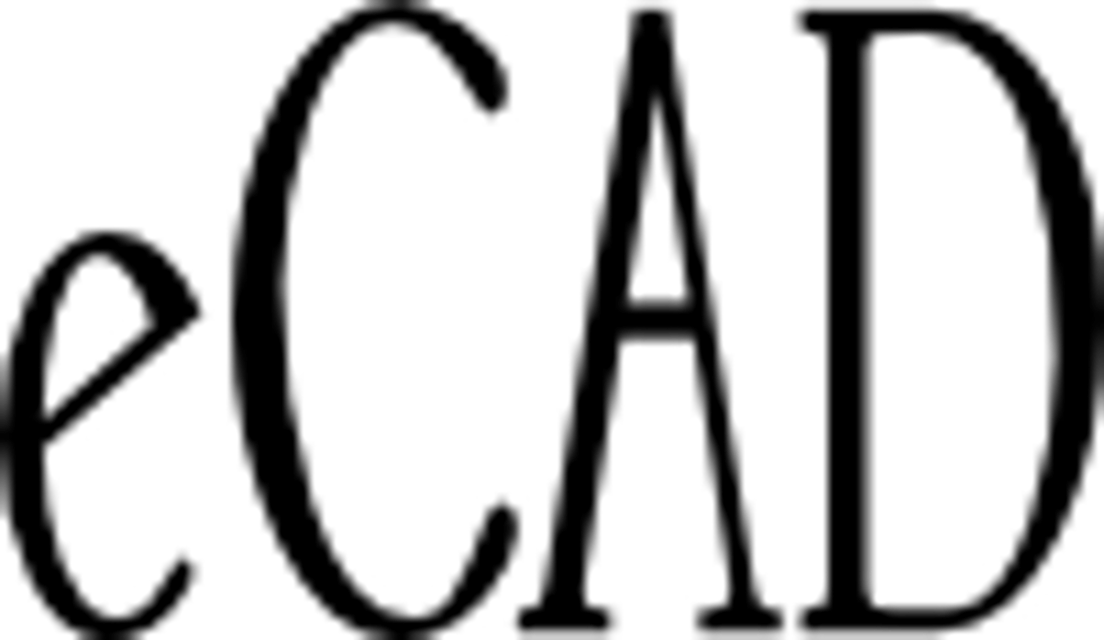
\includegraphics[width=0.7\textwidth]{images/logo.png}
\caption{eCAD logo}
\end{figure}
eCAD is a fully comprehensive 2D CAD application that you can download and install for free. It is available for major operating systems which includes Microsoft Windows and Linux. It is available in more than 20 languages and for major operating systems which includes Microsoft Windows and Linux.\\\\
The app is great for industrial designers, but anyone who wants to learn how to make 2D
CAD drawings will like this program. For a free software, eCAD gives you a lot of tools
to work with. New users will be able to create basic drawings, while advanced users can
make engineering plans with the software.You can start drawings from scratch. But it is
also easy to put in ellipses, arcs, lines and circles. eCAD also has a powerful zoom tool
that lets you look at models at different distances. This is essential for designers who
are going to make life size copies of a drawing. eCAD also has grids which are extremely
useful for those new to CAD. Once you have made the basic object, you can customize
it in many ways. Scaling is particularly easy here. Also Dimensioning which is must in
every CAD software is there. We can calculate the distance between two points and can
get the size of the object. Here, its worth mentioning about snapping part. We can have
snapping to grid, center etc. One if wants to work by writing a code can do so in scripting
feature. You can download and install eCAD freely, with no fear of copyright infringement.\\\\

\subsection{License}
\begin{figure}[h!]
\centering

\includegraphics[width=0.7\textwidth]{images/gpl.jpg}
\caption{GPLv3}
\end{figure}
The GNU General Public License is a free, copy left license for software and other kinds
of works. The licenses for most software and other practical works are designed to take
away your freedom to share and change the works. The GNU General Public License is a free, copy left license for software and other kinds
of works. The licenses for most software and other practical works are designed to take
away your freedom to share and change the works.\\\\
Then we speak of free software, we are referring to freedom, not price. Our General
Public Licenses are designed to make sure that you have the freedom to distribute copies
of free software (and charge for them if you wish), that you receive source code or can get
it if you want it, that you can change the software or use pieces of it in new free programs,
and that you know you can do these things. For example, if you distribute copies of such a program, whether gratis or for a fee,
you must pass on to the recipients the same freedoms that you received. You must make
sure that they, too, receive or can get the source code. And you must show them these
terms so they know their rights. Developers that use the GNU GPL protect your rights
with two steps:
\begin{itemize}
\item assert copyright on the software
\item offer you this License giving you legal permission to copy, distribute and/or modify
it.
\end{itemize}
For the developer’s and author’s protection, the GPL clearly explains that there is no
warranty for this free software. For both user’s and author’s sake, the GPL requires that
modified versions be marked as changed, so that their problems will not be attributed
erroneously to authors of previous versions.\\\\
For the developer’s and author’s protection, the GPL clearly explains that there is no
warranty for this free software. For both user’s and author’s sake, the GPL requires that
modified versions be marked as changed, so that their problems will not be attributed
erroneously to authors of previous versions.\\\\
Finally, every program is threatened constantly by software patents. States should not
allow patents to restrict development and use of software on general-purpose computers,
but in those that do, we wish to avoid the special danger that patents applied to a free
program could make it effectively proprietary. To prevent this, the GPL assures that
patents cannot be used to render the program non-free.\\\\




 

